\section{Análise gramatical}

\begin{frame}[fragile]{Análise gramatical}

    \begin{itemize}
        \item A análise gramatical é o processo de se determinar se uma cadeia de tokens pode ser gerada por uma gramática
        \pause

        \item O compilador deve ser capaz de construir uma árvore gramatical, mesmo que de forma implícita
        \pause

        \item Um analisador gramatical pode ser construído para qualquer gramática
        \pause

        \item Para qualquer gramáticas livres de contexto existe um analisador gramatical que analisa $N$ tokens com complexidade $O(N^3)$
        \pause

        \item Contudo, existem analisadores lineares para quase todas as gramáticas livres de contexto que surgem na prática
    \end{itemize}

\end{frame}

\begin{frame}[fragile]{Análise {\it top-down} e {\it bottom-up}}

    \begin{itemize}
        \item Há duas classes principais de analisadores gramaticais
        \pause

        \item Analisadores {\it top-down} a construção parte da raiz da árvore gramatical para suas folhas
        \pause

        \item Analisadores {\it bottom-up} partem das folhas em direção à raiz
        \pause

        \item Os analisadores \textit{top-down} são mais populares, pois é possível construir analisadores eficientes desta classe de forma manual
        \pause

        \item Já os analisadores \textit{bottom-up} podem manipular uma gama mais ampla de gramáticas
        \pause

        \item Geradores de analisadores gramaticais tendem a usar métodos \textit{bottom-up}
    \end{itemize}

\end{frame}

\begin{frame}[fragile]{Construção {\it top-down} de uma árvore gramatical}

    \begin{enumerate}
        \item Inicie na raiz, rotulada pelo não-terminal de partida
        \pause

        \item Repita os seguintes passos:
        \pause

        \begin{enumerate}[(a)]
            \item Para o nó $n$, rotulado pelo não-terminal $A$, selecione uma das produções para $A$ e construa os filhos de $n$ com os símbolos do lado
            direito da produção
            \pause

            \item Encontre o próximo nó no qual uma subárvore deve ser construída
        \end{enumerate}
    \end{enumerate}
    \pause

    \vspace{0.1in}
    Observações:
    \pause
    \begin{enumerate}[(i)]
        \item A depender da gramática, esta construção pode ser implementada com uma única passagem da entrada, da esquerda para a direita
        \pause

        \item O token que está sendo observado é frequentemente denominado \textit{lookahead}
        \pause

        \item Inicialmente \textit{lookahead} é o token mais à esquerda da entrada
    \end{enumerate}
\end{frame}

\begin{frame}[fragile]{Exemplo: gramática para geração de subtipos em Pascal}

\[
    \begin{array}{rcl}
        tipo & \to & primitivo \\
             & | & \uparrow \mathbf{id} \\
             & | & \mathbf{array}\ [\ primitivo \ ]\ \mathbf{of}\ tipo \\
        \\
        primitivo & \to & \mathbf{integer} \\
             & | & \mathbf{char} \\
             & | & \mathbf{num}\ ..\ \mathbf{num}
    \end{array}
\]
    \pause
    \vspace{0.2in}

    Observação: os dois pontos (`$..$') formam um único token.

\end{frame}

\begin{frame}[fragile]{Exemplo de construção {\it top-down} da árvore gramatical}

    Considere a expressão \code{pascal}{array [ num .. num ] of integer}, gerada a partir da gramática de subtipos em Pascal.
    \pause

    \vspace{0.2in}

    \begin{enumerate}[(a)]
        \item A construção inicial na raiz da árvore. O rótulo da raiz é o não-terminal de partida
        \pause

        \begin{center}
           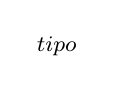
\begin{tikzpicture}
                \node (A) at (6, 6) { \footnotesize $tipo$ };
           \end{tikzpicture}
        \end{center}
        \pause

        \item A única produção de $tipo$ que inicia com o  \textit{lookahead} (neste momento, \code{pascal}{array}) é a terceira. Esta produção será
            usada para a criação dos filhos do nó raiz.
        \pause

        \begin{center}
           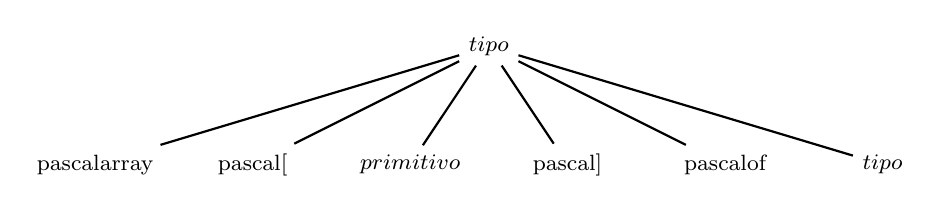
\begin{tikzpicture}
                \node (A) at (5, 5) { \footnotesize $tipo$ };
                \node (B1) at (0, 3.5) { \footnotesize \code{pascal}{array} };
                \node (B2) at (2, 3.5) { \footnotesize \code{pascal}{[} };
                \node (B3) at (4, 3.5) { \footnotesize $primitivo$ };
                \node (B4) at (6, 3.5) { \footnotesize \code{pascal}{]} };
                \node (B5) at (8, 3.5) { \footnotesize \code{pascal}{of} };
                \node (B6) at (10, 3.5) { \footnotesize $tipo$ };

                \draw[thick] (A) to (B1);
                \draw[thick] (A) to (B2);
                \draw[thick] (A) to (B3);
                \draw[thick] (A) to (B4);
                \draw[thick] (A) to (B5);
                \draw[thick] (A) to (B6);
           \end{tikzpicture}
        \end{center}

    \end{enumerate}
\end{frame}

\begin{frame}[fragile]{Exemplo de construção {\it top-down} da árvore gramatical}

    \begin{enumerate}[(a)]
        \setcounter{enumi}{2}
            \item O filho mais à esquerda tem como rótulo \code{pascal}{array}. Como este rótulo coincide com \textit{lookahead}, a construção prossegue para o
                próximo filho
            \pause

        \item \textit{Lookahead} é atualizado para \code{pascal}{[} e confrontado com o segundo filho à esquerda da raiz. Como há nova coincidência entre o rótulo
            e \textit{lookahead}, a construção prossegue
            \pause

        \item O nó seguinte contém o não-terminal $primitivo$ e \textit{lookahead} contém o token \code{pascal}{num}. Assim a terceira produção de $primitivo$
            é utilizada para gerar os novos filhos
        \pause

       \begin{center}
           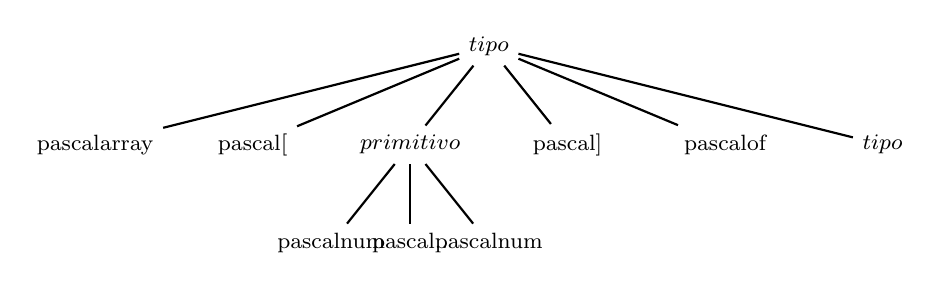
\begin{tikzpicture}
                \node (A) at (5, 5) { \footnotesize $tipo$ };
                \node (B1) at (0, 3.75) { \footnotesize \code{pascal}{array} };
                \node (B2) at (2, 3.75) { \footnotesize \code{pascal}{[} };
                \node (B3) at (4, 3.75) { \footnotesize $primitivo$ };
                \node (B4) at (6, 3.75) { \footnotesize \code{pascal}{]} };
                \node (B5) at (8, 3.75) { \footnotesize \code{pascal}{of} };
                \node (B6) at (10, 3.75) { \footnotesize $tipo$ };
                \node (C1) at (3, 2.5) { \footnotesize \code{pascal}{num} };
                \node (C2) at (4, 2.5) { \footnotesize \code{pascal}{..} };
                \node (C3) at (5, 2.5) { \footnotesize \code{pascal}{num} };

                \draw[thick] (A) to (B1);
                \draw[thick] (A) to (B2);
                \draw[thick] (A) to (B3);
                \draw[thick] (A) to (B4);
                \draw[thick] (A) to (B5);
                \draw[thick] (A) to (B6);
                \draw[thick] (B3) to (C1);
                \draw[thick] (B3) to (C2);
                \draw[thick] (B3) to (C3);

           \end{tikzpicture}
        \end{center}

    \end{enumerate}
\end{frame}

\begin{frame}[fragile]{Exemplo de construção {\it top-down} da árvore gramatical}

    \begin{enumerate}[(a)]
        \setcounter{enumi}{6}
        \item Os próximos tokens (\code{pascal}{:, num, of}) coincidem com os respectivos filhos
            \pause

        \item O último valor que \textit{lookahead} assum é \code{pascal}{integer}, o qual é confrontado com o filho mais à direita da raiz. Como o nó tem
            como rótulo o não-terminal $tipo$, a primeira produção deste deve ser usada para construir o novo nó, que por sua vez usa a primeira produção de
            $primitivo$ para construir seu único filho

        \pause
       \begin{center}
           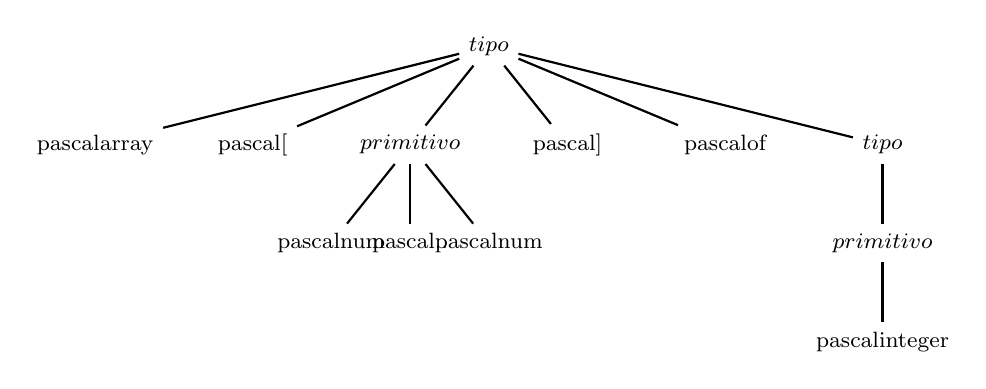
\begin{tikzpicture}
                \node (A) at (5, 5) { \footnotesize $tipo$ };
                \node (B1) at (0, 3.75) { \footnotesize \code{pascal}{array} };
                \node (B2) at (2, 3.75) { \footnotesize \code{pascal}{[} };
                \node (B3) at (4, 3.75) { \footnotesize $primitivo$ };
                \node (B4) at (6, 3.75) { \footnotesize \code{pascal}{]} };
                \node (B5) at (8, 3.75) { \footnotesize \code{pascal}{of} };
                \node (B6) at (10, 3.75) { \footnotesize $tipo$ };
                \node (C1) at (3, 2.5) { \footnotesize \code{pascal}{num} };
                \node (C2) at (4, 2.5) { \footnotesize \code{pascal}{..} };
                \node (C3) at (5, 2.5) { \footnotesize \code{pascal}{num} };
                \node (D1) at (10, 2.5) { \footnotesize $primitivo$ };
                \node (E1) at (10, 1.25) { \footnotesize \code{pascal}{integer} };

                \draw[thick] (A) to (B1);
                \draw[thick] (A) to (B2);
                \draw[thick] (A) to (B3);
                \draw[thick] (A) to (B4);
                \draw[thick] (A) to (B5);
                \draw[thick] (A) to (B6);
                \draw[thick] (B3) to (C1);
                \draw[thick] (B3) to (C2);
                \draw[thick] (B3) to (C3);
                \draw[thick] (B6) to (D1);
                \draw[thick] (E1) to (D1);

           \end{tikzpicture}
        \end{center}

    \end{enumerate}
\end{frame}

\begin{frame}[fragile]{Análise gramatical preditiva}

    \begin{itemize}
        \item Uma análise gramatical descendente recursiva é um método \textit{top-down} de análise sintática na qual são executados procedimentos recursivos
            para processar a entrada
        \pause

        \item Cada não-terminal da entrada é associado a um procedimento
        \pause

        \item Se \textit{lookahead} determina, sem ambiguidades, o procedimento a ser executado, a análise gramatical descendente recursiva é denominada
        análise gramatical preditiva
        \pause

        \item A sequência de chamadas de procedimentos no processamento da entrada determina, de forma implícita, a árvore gramatical
        \pause

        \item Além dos procedimentos associados aos não-terminais, a análise pode definir outros procedimentos auxiliares que podem simplificar tarefas como
            a leitura de tokens e a atualização de \textit{lookahead}
    \end{itemize}

\end{frame}

\begin{frame}[fragile]{Reconhecimento de tokens}

    O procedimento \Call{reconhecer}{\,} confronta o valor de \textit{lookahead} e um determinado token. Em caso de coincidência, ele atualiza \textit{lookahead} com
    o próximo token da entrada.
    \pause

    \vspace{0.2in}
    \begin{algorithmic}[1]
        \Procedure{reconhecer}{$token$}
        \Statex
        \If{$lookahead$ = $token$}
            \Comment{$lookahead$ é uma variável global}
            \State{$lookahead$ \gets \Call{proximoToken}{\,}}
        \Else
            \State{\Call{erro}{\,}}
        \EndIf
        \EndProcedure
    \end{algorithmic}
\end{frame}

\begin{frame}[fragile]{Procedimento associado ao não terminal $tipo$}

    \begin{algorithmic}[1]
        \Procedure{tipo}{\,}
        \If{$lookahead$ \code{apl}{∊} \{ \code{pascal}{integer, char, num} \} }
            \State{\Call{primitivo}{\,}}
        \ElsIf{$lookahead$ = $\uparrow$}
            \State{\Call{reconhecer}{$\uparrow$}}
            \State{\Call{reconhecer}{\code{pascal}{id}}}
        \ElsIf{$lookahead$ = \code{pascal}{array}}
            \State{\Call{reconhecer}{\code{pascal}{array}}}, \State{\Call{reconhecer}{\code{pascal}{[}}}
            \State{\Call{primitivo}{\,}}
            \State{\Call{reconhecer}{\code{pascal}{]}}}, \State{\Call{reconhecer}{\code{pascal}{of}}}
            \State{\Call{tipo}{\,}}
        \Else
            \State{\Call{erro}{\,}}
        \EndIf
        \EndProcedure
    \end{algorithmic}

\end{frame}

\begin{frame}[fragile]{Procedimento associado ao não terminal $primitivo$}

    \begin{algorithmic}[1]
        \Procedure{primitivo}{\,}
        \If{$lookahead$ = \code{pascal}{integer} }
            \State{\Call{reconhecer}{\code{pascal}{integer}}}
        \ElsIf{$lookahead$ = \code{pascal}{char}}
            \State{\Call{reconhecer}{\code{pascal}{char}}}
        \ElsIf{$lookahead$ = \code{pascal}{num}}
            \State{\Call{reconhecer}{\code{pascal}{num}}}
            \State{\Call{reconhecer}{\code{pascal}{:}}}
            \State{\Call{reconhecer}{\code{pascal}{num}}}
        \Else
            \State{\Call{erro}{\,}}
        \EndIf
        \EndProcedure
    \end{algorithmic}

\end{frame}

\begin{frame}[fragile]{Primeiros símbolos}

    \begin{block}{Definição de primeiros símbolos}
        Seja $\alpha$ o lado direito de uma produção. Então \Call{primeiro}{$\alpha$} é o conjunto de tokens que figuram como primeiros símbolos de uma ou mais
        cadeias geradas a partir de $\alpha$. Se \code{apl}{∊} pode ser gerado a partir de $\alpha$, então \code{apl}{∊} pertence a \Call{primeiro}{$\alpha$}.
    \end{block}

    \vspace{0.2in}
    Por exemplo, na gramática de geração de subtipos em Pascal,

    \begin{center}\Call{primeiro}{$primitivo$} = \{ \code{pascal}{integer, char, num} \}\end{center}

    e

    \begin{center}\Call{primeiro}{$\uparrow$\code{pascal}{id}} = \{ $\uparrow$ \}\end{center}

\end{frame}

\begin{frame}[fragile]{Primeiros símbolos e análise gramatica preditiva}

    \begin{itemize}
        \item A análise gramatical preditiva depende dos conjuntos \Call{primeiro}{$X$} de todos não-terminais $X$ da gramática
        \pause

        \item Isto acontece principalmente nos casos onde a gramática possui duas ou mais produções para um mesmo não-terminal (por exemplo, $A \to \alpha$ e
        $A\to \beta$)
        \pause

        \item Para que a análise gramatical recursiva descendente seja preditiva é necessário que os primeiros símbolos de cada produção sejam distintos
        \pause

        \item No exemplo dado,

        \begin{center}
        \Call{primeiro}{$\alpha$} $\cap$ \Call{primeiro}{$\beta$} = \emptyset
        \end{center}
        \pause

        \item Caso esta condição se verifique para todos os pares de produções distintas de um mesmo não-terminal, a produção $\gamma$ deve ser usada se
        $lookahead \in$ \Call{primeiro}{\gamma}
    \end{itemize}

\end{frame}

\begin{frame}[fragile]{Projeto de um analisador gramatical preditivo}

    Um analisador gramatical preditivo é um programa que contém um procedimento para cada não-terminal. Cada procedimento deve seguir dois passos:
    \pause

    \begin{enumerate}
        \item Determinar a produção a ser usada a partir de $lookahead$. Para tanto, deve ser localizada, entre as produções $\alpha_1, \alpha_2, \ldots, \alpha_N$,
            a produção $\alpha_i$ tal que $lookahead \in \Call{primeiro}{\alpha_i}$ (deve valer a seguinte propriedade: \Call{primeiro}{$\alpha_i$} $\cap$
            \Call{primeiro}{$\alpha_j$} = $\emptyset$ se $i\neq j$. Se $\alpha_k$ = \code{apl}{∊} para algum $k$, $\alpha_k$ deve ser usada se $lookahead$ não estiver
            presente em nenhuma outra produção
        \pause

        \item Identificada a produção, o procedimento imita a produção, reconhecendo os terminais da produção e chamandos os procedimentos dos não-terminais, na
            mesma ordem da produção
    \end{enumerate}

\end{frame}

\begin{frame}[fragile]{Produções recursivas à esquerda}

    \begin{block}{Definição de produção recursiva à esquerda}
        Uma produção é recursiva à esquerda se o não-terminal à esquerda da produção figura como primeiro símbolo da produção. Por exemplo, se $\alpha$ e $\beta$
        são sequências de terminais e não-terminais que não iniciam em $A$, então a produção
        \[
            A \to A\alpha\ |\ \beta
        \]
        é recursiva à esquerda.
    \end{block}
    \pause

    \vspace{0.2in}
    Observação: analisadores gramaticais recursivos descendentes pode rodar indefinidamente caso usem uma produção recursiva à esquerda
\end{frame}

\begin{frame}[fragile]{Produções recursivas à direita}

    \begin{block}{Definição de produção recursiva à direita}
        Uma produção é recursiva à direita se o não-terminal à esquerda da produção figura como último símbolo da produção. Por exemplo, se $\alpha$ e $\beta$
        são sequências de terminais e não-terminais que não terminam em $R$, então a produção
        \[
            \begin{array}{l}
            A \to   \beta R\\
            R \to   \alpha R\ |\ \code{apl}{∊}
            \end{array}
        \]
        é recursiva à direita.
    \end{block}
    \pause

    \vspace{0.2in}
    Observação: produções recursivas à direita dificultam a tradução de expressões que contém operadores associativos à esquerda
\end{frame}
